% !TeX spellcheck = nl_NL
\chapter{Functionality}\label{chap:functionality}
\begin{abstract}
If you like having a short abstract that summarises your chapters, you can add one with the \verb|abstract| environment.
%Did you ever hear the tragedy of Darth Plagueis The Wise? I thought not. It’s not a story the Jedi would tell you. It’s a Sith legend. Darth Plagueis was a Dark Lord of the Sith, so powerful and so wise he could use the Force to influence the midichlorians to create life… He had such a knowledge of the dark side that he could even keep the ones he cared about from dying. The dark side of the Force is a pathway to many abilities some consider to be unnatural. He became so powerful… the only thing he was afraid of was losing his power, which eventually, of course, he did. Unfortunately, he taught his apprentice everything he knew, then his apprentice killed him in his sleep. Ironic. He could save others from death, but not himself.
\end{abstract}

We just installed \repo in \autoref{chap:bauwemt}. Below, I showcase \emph{what} you can do with it. Because the source code for this documentation \emph{is} \repo, it shows you exactly \emph{how} to do everything that is showcased.


\section{Text style}
Paragraphs are separated by half a line of whitespace in \repo, and have no indents. In the source, you simply leave an empty line between paragraphs. No commands needed.

As usual in \LaTeX{}, it is recommended that you write what you \emph{mean}, not what to \emph{show}: don't ask "make this bold" but ask "emphasise this" and then later on decide that everything that is emphasised should be bolded (or slanted, or underlined, or made blue, etc...). In my thesis, I had commands for \emph{emphasis}, \co{code}, and \ex{examples}.

In some rare cases, you may want to hard-code the style. You can do that with:
\begin{center}
\begin{tabular}{l|l}
\bfseries Command form & \bfseries Series form \\ \hline
\verb|\textbf{...}|       & \verb|{\bfseries ...}| \\
\verb|\textit{...}|       & \verb|{\itshape ...}| \\  
\verb|\textsl{...}|       & \verb|{\slshape ...}| \\
\verb|\textsf{...}|       & \verb|{\sffamily ...}| \\
\verb|\textsc{...}|       & \verb|{\scshape ...}| \\
\verb|\textcolor{c}{...}| & \verb|{\color{c} ...}| \\ 
\verb|\underline{...}| & /
\end{tabular}
\end{center}

\section{Quotes}
\subsection{Inline quotes}
Normally, to balance quotes, you need \verb|``| and \verb|''|. This is annoying to type, and goes against the entire point of using \LaTeX{}, which again is to write what you \emph{mean}, not what to \emph{show}. Hence, \repo allows using \verb|"|, plain and simple.

\subsection{Block quotes}
To quote someone else's work correctly, it should be clear \emph{from where} and \emph{what exactly} was copied. For the latter, you can use quotation marks, but other markings work just as well. If you are Harvard's president, apparently you can water down these rules, as per \textcite{kettles_law_2023}:
\begin{blockquote}
	Harvard threatened to sue the New York Post for defamation over accusations of plagiarism against President Claudine Gay in October, calling the claims "demonstrably false." Then, the University’s own review found several instances of "duplicative language" in Gay’s work. \ellipsis Still, the summary of the review said the passages at issue, "while regrettable, did not constitute research misconduct," which had to involve "intentional deception or recklessness."
\end{blockquote}


\section{Language}
\repo comes pre-loaded with support for English and Dutch. Additionally, it provides support for including Greek (\textgreek{ὕβρις}), Russian (\textrussian{Правда}), and Hebrew (\texthebrew{יהוה}) characters, with the commands \verb|\textgreek|, \verb|\textrussian| and \verb|\texthebrew|.

You can change the main language at the top of \co{main.tex}. To adapt object names in the text (the actual "Figure", "Table", "Algorithm", ... that appears around the objects, and separately, the names used by \verb|\autoref| when referring to an object anywhere in the text) to a language that isn't English or Dutch, take a look at \directory{pre/Settings.tex}.

\section{Math}
%See \href{https://www.overleaf.com/learn/latex/Aligning_equations_with_amsmath}{this tutorial}. 
\repo comes with many math packages included so you don't have to look for what you need. See \autoref{tab:mathpackages} for the packages and their usages.

Please do your reader a favour by avoiding classic mistakes. Some of the things you should always do:
\begin{itemize}
	\item Use parentheses that adjust for height, like
	\begin{equation}
		\sin\left(\sum_{i=1}^{n} (x_i - y_i)^2 \right)^{\!1/2} \qquad\text{not}\qquad  \sin(\sum_{i=1}^{n} (x_i - y_i)^2 )^{1/2}.
	\end{equation}
	Also notice that \repo fixes bad spacing around big parentheses that you get by default in \LaTeX{}.

	\item Escape your operators: it's $\ln(x)$, $\sin(x)$, $\cos(x)$, $\softmax(x)$, ... not $ln(x)$, $sin(x)$, $cos(x)$, $softmax(x)$.

	\item Similarly, set text upright: it's $v_\text{max}$, not $v_{max}$.

	\item Number your equations (\emph*{Fischer's rule}), i.e.\ never use the \LaTeX{} environments \verb|equation*| or \verb|align*|. Perhaps you don't think a given equation deserves its own name, but what if someone wants to email you about it?

	\item Use punctuation after an equation if it ends a sentence, like
	\begin{equation}
		E = mc^2.
	\end{equation}
	Otherwise, you have sentences that are never actually ended anywhere.
\end{itemize}
The last two points were derived from a great essay by \textcite{mermin_whats_1989}. Famously, a paper that got over $\num{100000}$ citations in 5 years included (and still does) an equation that broke all of these guidelines at once (see page 6 of \cite{vaswani_attention_2017}).

\begin{table}[b]
\begin{tabular}{l|ll}
	\bfseries Package & \bfseries Why? & \bfseries Example \\ \hline
	\co{mathtools} 	& Math things & $\int$ \\
	\co{amssymb} 	& Fancier math things & $\mathbb{R}$ and $\mathcal{R}$ \\
	\co{dsfont} 	& Double-stroked letters & $\mathds{1}$ \\[-0.4em]
	\co{mathdots} 	& Dotty math things & $2^{2^{\iddots}}$ \\
	\co{bm} 		& Bold math & $\bm{W}$ \\
	\co{rsfso[scr]} & Sexy capitals & $\mathscr{L}$ \\
	\co{siunitx} 	& Units and scientific notation & $\num{6.022e23}$ and $\SI{9.81}{\metre\per\second\squared}$ \\
	\co{commath} 	& Derivative and integral d, and norms & $\pd{F}{x}$ and $F(x)\dif x$ and $\od{F}{x}$ \\
	\co{interval} 	& Intervals (semicolon, European brackets) & $\interval[open right]{0}{\infty}$ \\
\end{tabular}
\caption{\LaTeX{} packages already loaded in \repo for mathematical expression.}
\label{tab:mathpackages}
\end{table}


\subsection{Math examples}
\paragraph{Vectors and matrices} My notational convention is that vectors (\co{vec}) use the vector arrow, whilst matrices (\co{matr}) are bolded. For example, let there be $n$ words and their encoder embedding states $\vec h_e[1] \hdots \vec h_e[n] \in \R^H$. Now we define the relevance function $f : \R^H \times \R^H \to \R$ as a trainable FFNN, and the context vector $\vec c[t]$, as a weighted sum:
\begin{align}
	f(\vec h_e, \vec h_d) &= \matr W_o \tanh(\matr W_e \vec h_e + \matr W_d \vec h_d ) \label{eq:align}\\
	\vec \alpha[t] &= \softmax\left(\begin{bmatrix}f(\vec h_e[1], \vec h_d[t-1]) & \hdots & f(\vec h_e[n], \vec h_d[t-1])\end{bmatrix}\right) \\
	\vec c[t] &= \sum_{i=1}^{n} \alpha_i[t] \vec h_e[i] \label{eq:context}
\end{align}
where $\matr W_e, \matr W_d \in \R^{A\times H}$ and $\matr W_o \in \R^{1\times A}$, and $\vec h_d[t-1]$ is the previous decoder state.

Transformer cross-attention looks as follows: gather all the states of the encoder as the rows of two matrices $\matr K = \matr V \in \R^{n\times H}$, and those of the decoder in a matrix $\matr Q\in \R^{m\times H}$. In an attention head with weight matrices $\matr W_Q, \matr W_K, \matr W_V \in \R^{H\times d}$, we get:
\begin{equation}
	\text{Att}(\matr Q, \matr K, \matr V) = \softmax\left( \frac{(\matr Q\matr W_Q){(\matr K\matr W_K)}^\intercal}{\sqrt d} \right)(\matr V\matr W_V) \qquad \in \R^{m\times d}
\end{equation}
Vector norms:
\begin{align}
	\cos(\vec x, \vec y) &= \frac{\vec x \cdot \vec y}{\norm{\vec x} \norm{\vec y}} = \frac{\vec x}{\norm{\vec x}} \cdot \frac{\vec y}{ \norm{\vec y}} = \frac{\vec x}{\sqrt{\vec x\cdot \vec x}} \cdot \frac{\vec y}{ \sqrt{\vec y \cdot \vec y}} \\
	\vec x &= \tmatr W(\matr W\vec x) + \vec \varepsilon \qquad\text{with small } \norm{\vec \varepsilon}.
\end{align}
and so on.

\paragraph{Aligning equations} You can align equations in many ways, depending on whether you want to number all of the sub-equations or not. If you want the entire group of aligned equations to have one equation number, use an \co{aligned} inside an \co{equation}:
\begin{equation}\begin{aligned}
	\forall t\in V_{\theta'} : \dpd{}{p_t}\left(\sum_{t\in V_{\theta'}} C_{\D,{\theta'}}(t) \ln p_t - \lambda\left( \sum_{t\in V_{\theta'}} p_t - 1 \right) \right) &= 0 \\
	C_{\D,{\theta'}}(t) \dpd{}{p_t}\ln p_t - \lambda &= 0 \\
	p_t &= C_{\D,{\theta'}}(t)/\lambda 
\end{aligned}\end{equation}
For systems of equations, you can use \co{dcases}, which even works inside an \co{aligned}:
\begin{equation}\label{eq:mle}\begin{aligned}
	1 &= \sum_{t\in V_{\theta'}} p_t = \sum_{t\in V_{\theta'}} \frac{C_{\D,{\theta'}}(t)}{\lambda} = \frac{1}{\lambda}\sum_{t\in V_{\theta'}} C_{\D,{\theta'}}(t) = |\T_{\D,{\theta'}}|/\lambda \\
	&\text{and so }\; \begin{dcases}
		\lambda\hspace{-0.8em} &= |\T_{\D,{\theta'}}| \\
		p_t\hspace{-0.8em} &= C_{\D,{\theta'}}(t)/|\T_{\D,{\theta'}}| \quad(\forall t\in V)
	\end{dcases}
\end{aligned}\end{equation}
If you want to number all equations, and do so by advancing the equation number each time, use \co{align}:
\begin{align}
	F(xy) &= \sum_{w\in W_\D} \mathbb{I}\{C_{\theta'}(xy,w) > 0\}\, C_\D(w) \label{eq:modulatethis} \\
	\text{SFL}(\D) &= |X|\, \mathcal H(X) = |X|\sum_{t\in V\cup\{\co{,}\}}\!\! - \frac{C_X(t)}{|X|} \log_2\left( \frac{C_X(t)}{|X|} \right). \label{eq:sfl} \\
	\bm\theta_\text{MAP} &= \scalemath{0.95}{\arg\max_{\bm\theta} P(\bm\theta \mid \D) = \arg\max_{\bm\theta} \frac{P(\D \mid \bm\theta)P(\bm\theta)}{P(\D)} = \arg\max_{\bm\theta} P(\D \mid \bm\theta)P(\bm\theta)}. \label{eq:map} \\
	P(\Theta) &= P(|V|)\cdot |V|!\cdot \prod_{t\in V}\left[P_\Gamma(|t|)\prod_{c\in t} P(c)\right] \cdot \binom{|\T_{\D,\Theta}|-1}{|V|-1}^{\!-1} \label{eq:prior} \\
	P(\D\mid \Theta) &= \prod_{w\in W_\D}\left( P(K_{w,1}\mid K_0)\prod_{i=1}^{|\Theta(w)|} P(K_{w,i+1}\mid K_{w,i}) P(t_{w,i} \mid K_{w,i} ) \right)^{\!\!C_\D(w)} \label{eq:hmm}
\end{align}
If you want to split an equation inside \co{align}, wrap it inside \co{split}. The ampersands inside \co{split} will align with those in \co{align}.
\begin{align}
	\begin{split}
		\Li(\D;\Theta) &= \ln P(\D \mid \Theta) = \ln \prod_{s\in\D} \sum_{\zeta\in \mathcal S_V(s)} P(\zeta,s\mid \Theta) \\
		&= \sum_{s\in\D} \ln\left(\sum_{\zeta\in \mathcal S_V(s)} P(\zeta,s\mid \Theta)\right) 
	\end{split} \\
	P(\D \mid \Theta) &= \prod_{s\in \D} P(s \mid \Theta) = \prod_{s\in\D} \sum_{\zeta\in \mathcal S_V(s)} P(\zeta,s\mid \Theta) = \prod_{s\in\D} \sum_{\zeta\in \mathcal S_V(s)} \prod_{t\in \zeta} p_t \label{eq:kudo} \\
	\begin{split}
		\Delta\mathcal L(s;\Theta)[t] &= \ln\left(\sum_{\zeta\in \mathcal S_V(s)} P(\zeta,s\mid \Theta)\right) - \ln\left(\sum_{\zeta\in \mathcal S_V(s) \mid t\notin \zeta} P(\zeta,s\mid \Theta)\right) \\ 
		&= \ln(P_s) - \ln\left(P_s - \sum_{\zeta\in \mathcal S_V(s) \mid t\in \zeta} P(\zeta,s\mid \Theta)\right)
	\end{split}
\end{align}
Common mistakes when using \co{align} are blank lines around or inside the environment. Blank lines around it cause extra spacing, blank lines inside it cause errors.

Multiple ampersands in the same equation alternate between being \emph{points of alignment} and \emph{points to insert space}.
\begin{align}
	\text{muggenziften:}& & &\texttt{\small ((mug)[N],(e)[V|N.V],(zift)[V])[V]} \\
	\text{krokodillentranen:}& & &\texttt{\small((krokodil)[N],(e)[N|N.N],(traan)[N])[N]}.
\end{align}
If you don't want equation numbers, use \co{align*}, or \co{equation*} with \co{aligned}.
\begin{align*}
	\text{MUV}(\tau) &= -\frac{(\mathcal H(\tau + \Delta\tau) - \mathcal H(\tau))}{\Delta\tau} \qquad\text{with $\tau\in\N$ and $\Delta\tau\in\N$}, \\
	\text{PMI}(w_1,w_2) &= \frac{P(w_1,w_2)}{P(w_1)P(w_2)} \stackrel{\text{MLE}}{\propto} \frac{C_\D(w_1w_2)}{C_\D(w_1)C_\D(w_2)}
\end{align*}
If you want to take away only one label, use \verb|\nonumber| after an equation.
\begin{align}
	\text{score}(s_1,\hdots,s_m) &= \sqrt[m]{\prod_{i=1}^m C_{\D}(s_i)} = \exp\left(\frac{1}{m}\sum_{i=1}^{m}\ln C_{\D}(s_i)\right) \label{eq:knk} \nonumber \\
	P(\D \mid \Theta) &= \prod_{i=1}^{|\T_{\D,\Theta}|} P(t_i\mid t_{i-1},\hdots,t_{i-N+1})
\end{align}
but for both this and the above, beware of Fischer's rule.

\begin{subequations}
Surround regions of your text by \verb|\begin{subequations}...\end{subequations}| whenever you want the equation number to stay the same and instead count up a sub-number. For example,
\begin{equation}
	ax^2 + bx + c = 0
\end{equation}
is equivalent to
\begin{equation}
	x = \frac{-b \pm \sqrt{b^2 - 4ac}}{2a}
\end{equation}
and therefore it is reasonable to use sub-numbering.
\end{subequations}

Lastly, \repo has an extra environment \verb|subequations*| that picks up where the previous \verb|subequations|/\verb|subequations*| left off. For example, we could have a new equation
\begin{equation}
	(x - a)^2 + (y - b)^2 = c^2
\end{equation}

\begin{subequations*}
and then circle back to 
\begin{equation}
	D = b^2 - 4ac = (2ax + b)^2
\end{equation}
and so on.
\end{subequations*}

\paragraph{Scaling and shifting} You can use \verb|\scalemath{factor}{...}| inside an equation to make the math smaller without making the label smaller. You can nudge equations horizontally by some distance \co{d} by prefixing them with \verb|\hspace{d}|. You can space out equations vertically by some extra distance \co{d} by suffixing the \verb|\\| between them with \verb|[d]| like this:
\begin{equation}\hspace{-2em}\scalemath{0.7}{\begin{aligned}
	P &= \frac{\text{TP}}{\text{TP} + \text{FP}} = \frac{\#(\text{correct gesplitst} \mid \text{te splitsen})}{\text{TP} + \#(\text{fout gesplitst} \mid \text{te splitsen}) + \#(\text{gesplitst} \mid \text{niet te splitsen})} \\[0.75em]
	R &= \frac{\text{TP}}{\text{TP} + \text{FN}} = \frac{\#(\text{correct gesplitst} \mid \text{te splitsen})}{\text{TP} + \#(\text{fout gesplitst} \mid \text{te splitsen}) + \#(\text{niet gesplitst} \mid \text{te splitsen})} 
\end{aligned}}\end{equation}

\section{Hyperlinks}\label{sec:hyperlinks}
Internal references, i.e.\ links that jump to objects in the document (chapters, sections, captioned figures and tables, ...) should be made with \verb|\autoref| after having put a \verb|\label| inside or after such an object (or its caption). External references are added with \verb|\href|. This is less recommended in a paper thesis, because it will hide the URL. \verb|\url| also works. See \href{https://academia.stackexchange.com/q/195802/124578}{this post} for a discussion about whether that's good or bad.

\repo contains extra linking features that don't come with \LaTeX{} by default: 
\begin{itemize}
	\item You can \verb|\autoref| to individual lines in algorithms, like \autoref{line:bpeargmax} in \autoref{algo:bpe}.
	\item You can include the name of the object itself with the new command \verb|\fullref|, like \fullref{sec:hyperlinks}.
	\item You can link to the exact page of a label placed in running text by using the new command \verb|\pagelabel| and then using the existing command \verb|\autopageref|. By default, \LaTeX{} will output the correct page number, but an incorrect link: for example, I described what \co{main.tex} does on \autopageref{page:maintex} (link to a \verb|\pagelabel|) which is not what \LaTeX{} links to when it says \autopageref{page:maintex-wrong} by default (link to the \verb|\label| right next to it).
\end{itemize}
Also, as you may have noticed, \repo styles section references with \verb|\autoref| as "\S..." rather than "section ..." which looks much cleaner.

\section{Bibliography}
After you have exported a \co{.bib} file from your reference manager (preferably \textsf{Zotero}), have dropped it under \directory{res/bib/} and have declared this file with an \verb|\addbibresource| command in \directory{pre/Bibliography.tex}, you can use all your Bib\TeX{} tags in the following commands that come with Bib\LaTeX{} by default:

\begin{tabular}{llp{6.5cm}}
	\bfseries Command & \bfseries Output format & \bfseries Example output \\\hline
	\verb|\textcite{}| & Name (year) & \textcite{bauwens_bpe-knockout_2023} \\
	\verb|\parencite{}| & (Name, year) & \parencite{bauwens_bpe-knockout_2023} \\
	\verb|\cite{}| 	    & Name, year & \cite{bauwens_bpe-knockout_2023} \\
	\verb|\cites{}{}...|   & Name\textsubscript1, year\textsubscript1; Name\textsubscript2, year\textsubscript2; ... & \cites{bauwens_bpe-knockout_2023}{mermin_whats_1989} \\\hline 
	
	\verb|\citeauthor{}| & Name & \citeauthor{bauwens_bpe-knockout_2023} \\
	\verb|\citeyear|	 & year &  \citeyear{bauwens_bpe-knockout_2023} \\
	\verb|\citetitle{}| & "Title" & \citetitle{bauwens_bpe-knockout_2023}
\end{tabular}

\repo has an extra command \verb|\textcitefirst{}| to show only the first author and hiding the others under "et al".

The exact way in which citations and the bibliography at the ends of the thesis are rendered, is documented in \directory{pre/Imports.tex} and \directory{pre/Bibliography.tex}.

\section{Index}
\repo comes with support for an \emph*{index} of key terms. When you \verb|\emph|asise a term, you can choose to add an asterisk to the command so that the string that was emphasised also appears in a list all the way at the end of the thesis along with its page number: if the term \emph{is} capitalised \emph{and} you want to \emph{keep} that first capital letter in the index, use \verb|\Emph*{...}|. Otherwise (the more usual case), use \verb|\emph*{...}|.

You can also quietly add terms to the index using \verb|\index{...}| in the relevant location.

\begin{mdframed}
\textbf{Important:} Unless TeXstudio has a special setup for compiling your index, it is not updated even after saving and compiling the thesis with new \verb|\emph*| calls added. Make sure that after you have finished writing your thesis, you click on \menu[,]{Tools,Index} to regenerate the index manually.
\end{mdframed}


\section{Floats}
Floats are chunks in your thesis whose precise position is not that important -- they float somewhere around where you define them.

Floats have an alignment property that can be \co{h} (around \emph{h}ere), \co{t} (at the \emph{t}op of a nearby page), \co{b} (at the \emph{b}ottom of a nearby page), \co{p} (on a \emph{p}age dedicated to only floats), or \co{H} for stopping it from floating at all (exactly \emph{H}ERE).

Floats have a caption that shows up in one of the lists that follow the table of contents. For some floats, you'll want to use two captions like \verb|\caption[cap1]{cap2}|, where the first lands in the list and the second is displayed under the float.

\subsection{Figures}
\subsubsection{Regular image file}
\begin{figure}[h]
	\centering
 	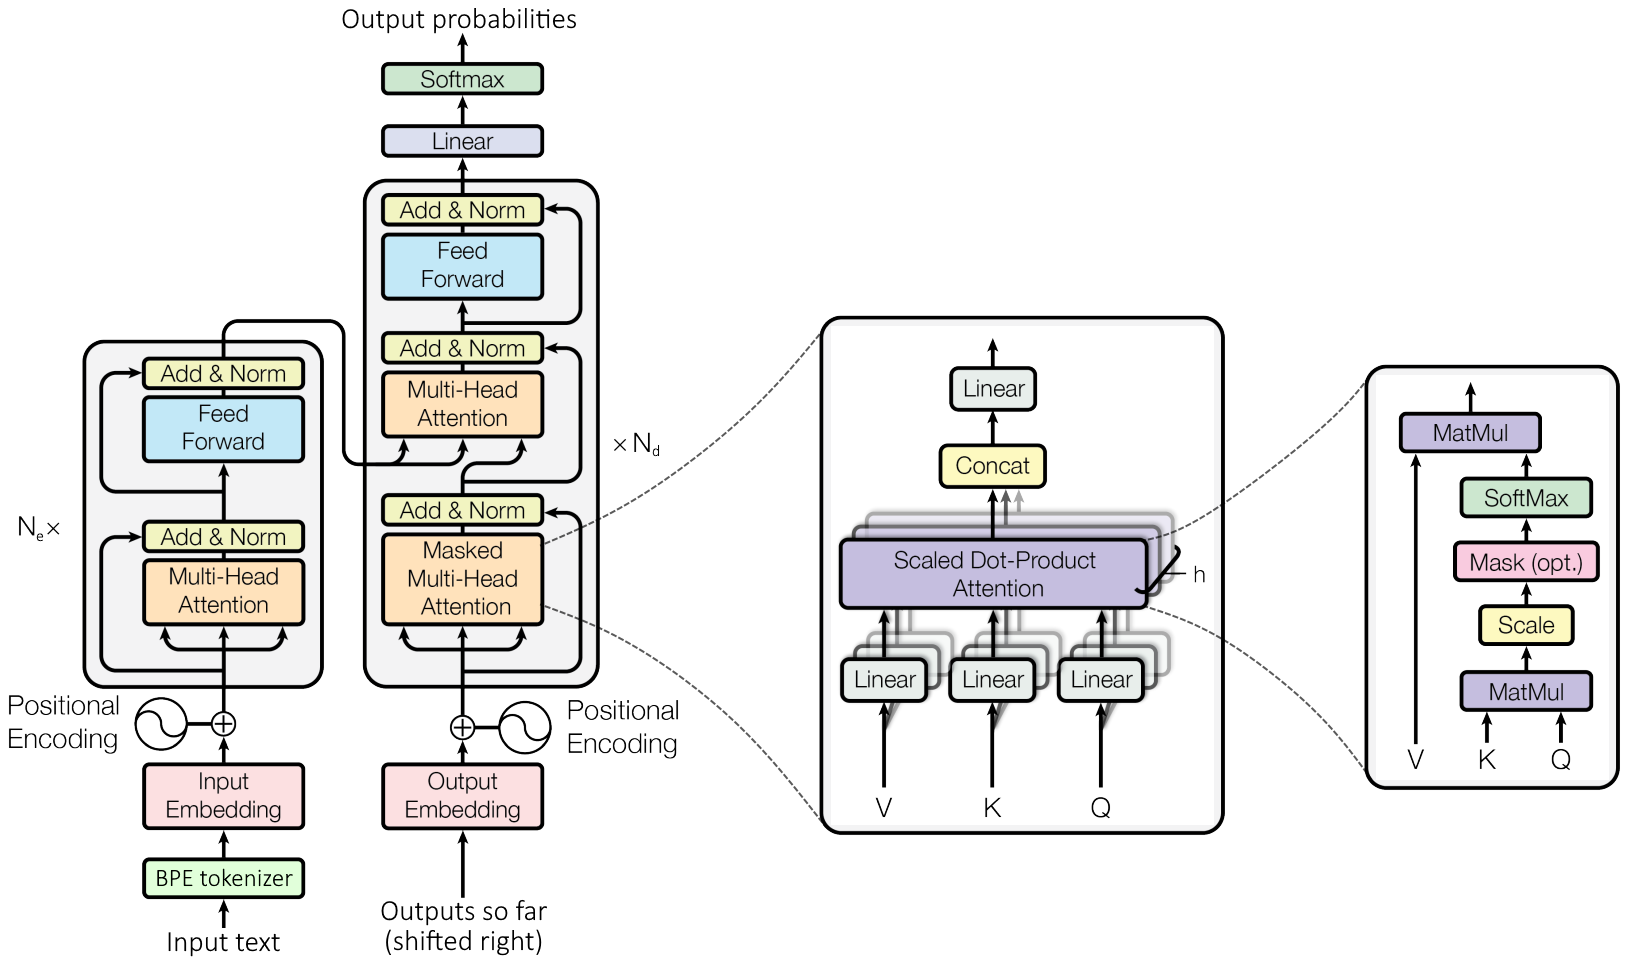
\includegraphics[width=\linewidth]{res/fig/vaswani-transformer}
	\caption[The transformer architecture]{The transformer architecture. Combination of figures by \textcite{vaswani_attention_2017}.}
	\label{fig:transformer}
\end{figure}

\newpage

\subsubsection{Embedded Ti$k$Z code}
\begin{figure}[H]
	\centering
	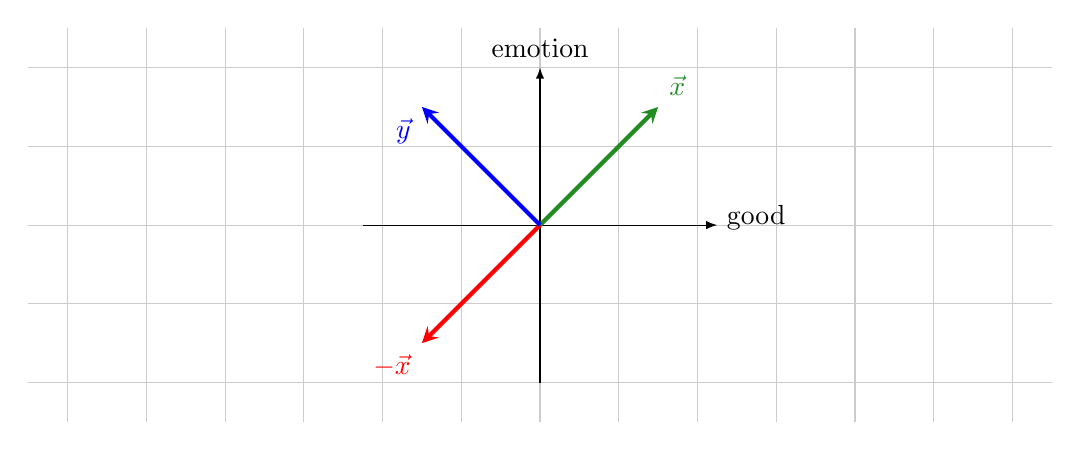
\begin{tikzpicture}[>=latex] 
		\draw[thin,gray!40] (-6.5,-2.5) grid (6.5,2.5);
		\draw[->] (-2.25,0)--(2.25,0) node[right,yshift=1mm]{good};
		\draw[->] (0,-2)--(0,2) node[above]{emotion};
		\draw[line width=1.5pt,ForestGreen,-stealth](0,0)--(1.5,1.5) node[anchor=south west]{$\vec x$};
		\draw[line width=1.5pt,red,-stealth](0,0)--(-1.5,-1.5) node[anchor=north east]{$-\vec x$};
		\draw[line width=1.5pt,blue,-stealth](0,0)--(-1.5,1.5) node[anchor=north east]{$\vec y$};
	\end{tikzpicture} 
	\caption{Small example of a Cartesian grid in Ti$k$Z.}
	\label{fig:semanticalgebra}
\end{figure}


\subsubsection{Subfigures}
\begin{figure}[h]
	\begin{subfigure}{0.5\linewidth}
		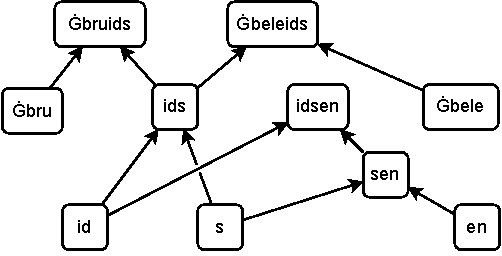
\includegraphics[width=\linewidth]{./res/fig/knockout-before}
		\caption{Before}
	\end{subfigure}
	\hspace{2em}
	\begin{subfigure}{0.5\linewidth}
		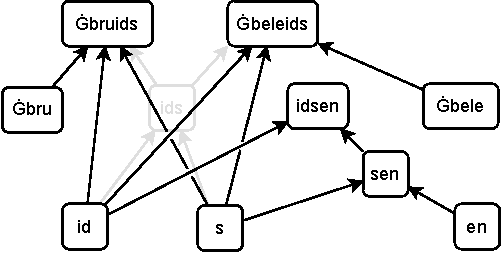
\includegraphics[width=\linewidth]{./res/fig/knockout-after}
		\caption{After}
	\end{subfigure}
	\caption[Visualisation of BPE-knockout]{Visualisation of the changes in part of the BPE merge graph after knockout of the Dutch type \ex{ids}, originating from the merge \ex{id+s}.}
	\label{fig:knockout}
\end{figure}

\begin{landscape}
\mbox{}\vfill 

\subsection{Tables}

\begin{table}[H]
\centering 
\scalebox{0.95}{
\begin{tabular}{c|rr:rr|rr:rr}
                        & \multicolumn{4}{c|}{\thead{morfen}} & \multicolumn{4}{c}{\thead{morfemen}} \\
                        & \thead{gevaren}  & \thead{$\%_\text{tot}$} & \thead{effectief}   & \thead{$\%_\text{gev}$}  & \thead{gevaren}   & \thead{$\%_\text{tot}$} & \thead{effectief}   & \thead{$\%_\text{gev}$}   \\ \hline
\multicolumn{1}{r|}{FP} & $\num{147622}$  &    $61.85\%$    & $\num{16015}$         & $10.85\%$   &  $\num{123743}$    & $51.7\%$     & $\num{11642}$         & $9.41\%$    \\
\multicolumn{1}{r|}{FN} & $\num{16860}$   & $7.06\%$      & $\num{5787}$         & $34.32\%$   & $\num{10077}$    & $4.21\%$     & $\num{2903}$         & $28.81\%$
\end{tabular}
}
\caption[Positive and negative prefix aliasing in e-Lex.]{Positive and negative prefix aliasing in e-Lex. "Hazards" refers to the amount of morphs or morphemes that risk being aliased, and "effective" refers to how many of those materialise while using BPE.}
\label{tab:aliasing}
\end{table}


\begin{table}[h]
\centering 
\scalebox{0.95}{
\begin{tabular}{r|cccccccc}
   & \multicolumn{2}{c|}{\thead{deletie}}        & \multicolumn{2}{c|}{\thead{substitutie}}    & \multicolumn{2}{c|}{\thead{wisseling}}      & \multicolumn{2}{c}{\thead{insertie}}       \\
   & e-Lex & \multicolumn{1}{c|}{NT2Lex} & e-Lex & \multicolumn{1}{c|}{NT2Lex} & e-Lex & \multicolumn{1}{c|}{NT2Lex} & e-Lex & \multicolumn{1}{c}{NT2Lex} \\ \hline 
	Pr & 0.58 & 0.38 & 0.50 & 0.32 & 0.44 & 0.28 & 0.46 & 0.30 \\
	Re & 0.79 & 0.78 & 0.87 & 0.87 & 0.80 & 0.80 & 0.89 & 0.89 
\end{tabular}
}
\caption{Precision en recall van de splitsingspunten die de BPE-tokeniser ingelast in woorden met typo's t.o.v.\ zonder.}
\label{tab:typos}
\end{table}

\begin{table}[h]
\centering
\resizebox{0.8\linewidth}{!}{
\begin{tabular}{lccr|cccccc|cccccc}
& \multirow{3}{*}{\rotatebox{90}{\bfseries Knockout}}& \multirow{3}{*}{\rotatebox{90}{\bfseries Anneal}} &       & \multicolumn{6}{c|}{\thead{morfemen}}                                   & \multicolumn{6}{c}{\thead{lexemen}}                                    \\
&&&       & \multicolumn{3}{c|}{\thead{types}}        & \multicolumn{3}{c|}{\thead{tokens}} & \multicolumn{3}{c|}{\thead{types}}        & \multicolumn{3}{c}{\thead{tokens}} \\
&&& $|V|$ & \thead{Pr} & \thead{Re} & \multicolumn{1}{c|}{\thead{$F_1$}} & \thead{Pr}      & \thead{Re}      & \thead{$F_1$}      & \thead{Pr} & \thead{Re} & \multicolumn{1}{c|}{\thead{$F_1$}} & \thead{Pr}      & \thead{Re}      & \thead{$F_1$}     \\ \hline
BTE & -- & -- & 40.0k & \tgrad{0.52} & \tgrad{0.55} & \multicolumn{1}{c|}{\tgrad{0.54}} & \tgrad{0.55} & \tgrad{0.12} & \multicolumn{1}{c|}{\tgrad{0.19}} & \tgrad{0.38} & \tgrad{0.70} & \multicolumn{1}{c|}{\tgrad{0.50}} & \tgrad{0.36} & \tgrad{0.31} & \tgrad{0.33} \\
BTE-knockout & L & -- & 38.4k & \tgrad{0.56} & \tgrad{0.62} & \multicolumn{1}{c|}{\tgrad{0.59}} & \tgrad{0.68} & \tgrad{0.24} & \multicolumn{1}{c|}{\tgrad{0.35}} & \bfseries \tgrad{0.43} & \tgrad{0.82} & \multicolumn{1}{c|}{\bfseries \tgrad{0.56}} & \bfseries \tgrad{0.56} & \tgrad{0.79} & \bfseries \tgrad{0.66} \\
BTE-knockout-notrivial & L & -- & 39.5k & \tgrad{0.55} & \tgrad{0.61} & \multicolumn{1}{c|}{\tgrad{0.58}} & \tgrad{0.57} & \tgrad{0.15} & \multicolumn{1}{c|}{\tgrad{0.23}} & \tgrad{0.42} & \tgrad{0.80} & \multicolumn{1}{c|}{\tgrad{0.55}} & \tgrad{0.41} & \tgrad{0.42} & \tgrad{0.41} \\
BTE-knockout & M & -- & 35.7k & \bfseries \tgrad{0.61} & \bfseries \tgrad{0.78} & \multicolumn{1}{c|}{\bfseries \tgrad{0.69}} & \bfseries \tgrad{0.82} & \bfseries \tgrad{0.65} & \multicolumn{1}{c|}{\bfseries \tgrad{0.72}} & \tgrad{0.38} & \bfseries \tgrad{0.83} & \multicolumn{1}{c|}{\tgrad{0.52}} & \tgrad{0.26} & \bfseries \tgrad{0.82} & \tgrad{0.39} \\
BTE-knockout-notrivial & M & -- & 37.7k & \tgrad{0.60} & \tgrad{0.73} & \multicolumn{1}{c|}{\tgrad{0.66}} & \tgrad{0.72} & \tgrad{0.38} & \multicolumn{1}{c|}{\tgrad{0.49}} & \tgrad{0.38} & \tgrad{0.80} & \multicolumn{1}{c|}{\tgrad{0.51}} & \tgrad{0.20} & \tgrad{0.42} & \tgrad{0.28} \\
\end{tabular}}
\caption{Evaluatie van BPE-knockout op morfemische en lexemische splitsingspunten in e-Lex.}
\label{tab:knockouttrivial}
\end{table}

\vfill
\end{landscape}

If you want to have tables with numerical results that are within a certain range where one end is good and the other end is bad, you can surround each cell with the \verb|\tgrad{...}| command (short for \emph{table gradient}) to colour the background. One example of such a table is \autoref{tab:knockouttrivial}. Another can be found on page 9 of \textcite{bauwens_bpe-knockout_2024}. If your results originate from a Python program, I highly recommend you use the \href{https://github.com/bauwenst/fiject}{\textsf{fiject}} package to generate your table, including the wrapping of the cells, automatically.
 
\subsection{Algorithms}
Algorithms are floats containing a (non-floating) \verb|algorithmic| environment preceded by a caption and a label. They are numbered automatically, like figures.

To refer to a specific line in a specific algorithm, just put a \verb|\label| at the end of that line and \verb|\autoref| to it. \repo will make sure that the resulting reference links back to the correct line of the correct algorithm.

\autoref{algo:bpe} is a basic algorithm.
\begin{algorithm}[H]
	\caption{Pseudocode BPE}
	\label{algo:bpe}
	\begin{algorithmic}[1]
		\Function{leerBPE}{$\D$, $\tau$}
			%\State Comprimeer $\D$ tot de woordaantallen $W$.
			%\State Splits de woorden in $W$ in karakters, en voeg telkens een EOW-karakter toe.
			\State $\D \gets$ \Call{splitsInWoorden}{$\D$}
			\State $\D \gets$\texttt{[}\Call{splitsInLetters}{$w$} + \texttt{[}\textsc{eow}\texttt{]} $\mid w\in \D$\texttt{]} 
			\State $V \gets \{\ell \in w \mid w \in \D\}$\label{line:bpeinit}
			\State $M \gets \texttt{[]}$
			\While{$|V| < \tau$}
				\State $(x,y) \gets \arg\max\limits_{x,y\in V}$ \Call{aantal}{$\D$, $x$\_$y$}\label{line:bpeargmax}
				\State $\D\gets$ \Call{vervang}{$\D$, $x$\_$y$, $xy$}\label{line:replace}
				\State $V\gets V \cup \{xy\}$
				\State $M\gets M + \texttt{[}(x,y)\texttt{]}$
			\EndWhile
			\vspace{-0.31em}\State\Return $(V,M)$
%			\Stateh\Return $(V,M)$
		\EndFunction
	\end{algorithmic}
\end{algorithm}

You can colour parts of algorithms if you want to highlight them, like in \autoref{algo:bpedropout}.
\begin{algorithm}[H]
	\caption{Pseudocode BPE-dropout}
	\label{algo:bpedropout}
	\begin{algorithmic}[1]
		\Function{gebruikBPEdropout}{$V$, $M$, $w$, $p$}
			\State $w\gets$ \Call{splitsInLetters}{$w$} + \texttt{[}\textsc{eow}\texttt{]}
			\State $i\gets 0$
			\While{$i < |M|$}
				\State $(x,y) \gets M[i]$
				\State $i \gets i + 1$   % i never goes down again.
				\If{$x$\_$y \in w$}
					{\color{blue}
					\If{\Call{random}{0,1} $ < p$}
						\State $w \gets$ \Call{vervang1}{$w$, $x$\_$y$, $xy$}
						\State $i \gets 0$
					\EndIf
					}
				\EndIf
			\EndWhile
			\Statey \Return \texttt{[}\Call{index}{$V$, $t$} $\mid t \in w$\texttt{]}
		\EndFunction
	\end{algorithmic}
\end{algorithm}

\newpage

You can also space out two lines by putting a \verb|\vspace| in between them, like I do to separate two functions in \autoref{algo:kudo}.
\begin{algorithm}[H]
	\caption{Pseudocode ULM}
	\label{algo:kudo}
	\begin{algorithmic}[1]
		\Function{leerULM}{$\D$, $\tau$, $\eta$}
			\State $V \gets $ \Call{alleSubstrings}{$\D$}
			\State $\vec p = (p_1,\hdots,p_{|V|}) \gets (\tfrac{1}{|V|},\hdots,\tfrac{1}{|V|})$
			\While{$|V| > \tau$}
				\State $\vec p \gets$ \Call{herschat}{$\D$, $V$, $\vec p$}
				\State $\Delta\vec{\mathcal L} \gets \vec 0$\Comment{Totale log-likelihoodafname per type}
				\For{$s\in \D$}
					\State $P_s \gets 0$
					\State $\Delta\vec{P}_s \gets \vec 0$  \Comment{Kansafname in $s$ per type}
					\For{$\zeta \in$ \Call{segmentaties}{$s$, $V$}}
						\State $P_\zeta \gets \displaystyle\prod_{t\in \zeta} p_t$\label{line:ulm}  \Comment{Kans van de zinsegmentatie...}
						\State $P_s \gets P_s + P_\zeta$
						\For{$t\in \zeta$}
							\State $\Delta\vec{P}_s[t] \gets \Delta\vec{P}_s[t] + P_\zeta$  \Comment{...valt weg als $t$ wegvalt.}
						\EndFor
					\EndFor 
					\Stateh $\Delta\vec{\mathcal L} \gets \Delta\vec{\mathcal L} + \ln(P_s) - \ln(P_s - \Delta\vec P_s)$  
				\EndFor
				\Statey $V\gets$ \Call{sorteerAflopend}{$V$, $\Delta\vec{\mathcal L}$}  
				\State $V \gets V$\co{[}$0:\eta|V|$\co{]}  \Comment{Weinig likelihood weggevallen $\Rightarrow$ niet nodig}
			\EndWhile
			\Statey \Return $(V,\vec p)$
		\EndFunction
		\vspace{1em}
		\Function{gebruikULM}{$w$, $V$, $\vec p$}
			\State \textsl{Voorwaartse fase (iteratieve i.p.v.\ recursieve viterbi):}
			%\State $m\gets \max\{|t| \mid t\in V\}$
			\State $\ell_1 \hdots \ell_{|w|} \gets -\infty$  \Comment{Beste score tot nu toe gezien door substring $w$\listindex{$1:i$}}
			\State $t_1 \hdots t_{|w|} \gets \unk$  \Comment{Beste eindtoken tot nu toe voor substring $w$\listindex{$1:i$}}
			\For{$i = 1\hdots |w|$}
				%\For{$j = i+1\hdots \min\{i+m, |w|\}$}
				\For{$j = i+1\hdots |w|$}
					\State $t\gets w$\listindex{$i:j$} 
					\If{$t\in V$}
						\State $\ell \gets\ell_i + \ln p_t$
						\If{$\ell > \ell_j$}
							\State $\ell_j \gets \ell$
							\State $t_j \gets t$
						\EndIf 
					\EndIf 
				\EndFor 
			\EndFor 
			\Stateh \textsl{Achterwaartse fase (viterbi-tracé):}
			\State $T\gets$ \co{[]}
			\State $i\gets |w|$
			\While{$i > 0$}
				\State $T \gets$ \co{[}$t_i$\co{]} + $T$
				\State $i \gets i - |t_i|$
			\EndWhile
			\Statey \Return $T$
		\EndFunction
	\end{algorithmic}
\end{algorithm}

\repo defines the two algorithm commands \verb|\Statey| and \verb|\Stateh| which are necessary at some points in an algorithm to connect the indent lines together (e.g.\ after an early return statement). See examples in the source code of \autoref{algo:knockout}.
\begin{algorithm}[H]
	\caption{Knockout: verwijdering van een type uit de BPE-mergegraaf}
	\label{algo:knockout}
	\begin{algorithmic}[1]
		\Function{knockout}{$V$, $M_i$, $M_o$, $\ft$}
			\If{$|M_i(\ft)| = 0$} \Comment{$\ft$ deel van het alfabet}
				\State\Return $(V, M_i, M_o)$
			\EndIf
			\Statey $\{m_\text{old}\} \gets M_i(\ft)$
			\State $o_1,\hdots, o_n \gets$ \Call{ouders}{$m_\text{old}$}
			\For{$i \in 1\hdots n$}
				\State $M_o(o_i) \gets M_o(o_i) \setminus \{m_\text{old}\}$  \Comment{elke ouder vormt $\ft$ niet meer}
			\EndFor \vspace{-0.22em}
			\ForAll{$(q,(t_1, \hdots, \ft, \hdots, t_m)) \in M_o(\ft)$}
				\State $m_\text{new} \gets (q, (t_1,\hdots, o_1, \hdots, o_n, \hdots, t_m))$
				\State $M_i(t_1\hdots \ft \hdots t_m) \gets \{m_\text{new}\}$  \Comment{kind van $\ft$ gevormd door nieuwe merge}
				\For{$i \in 1\hdots n$}
					\State $M_o(o_i) \gets M_o(o_i) \uni\, \{m_\text{new}\}$  \Comment{elke ouder van $\ft$ vormt nu dit kind}
				\EndFor
			\EndFor
			\Statey $V \gets V \setminus \{\ft\}$
			\State $M_i(\ft) \gets \{\}$
			\State $M_o(\ft) \gets \{\}$
			\State \Return $(V, M_i, M_o)$
		\EndFunction
	\end{algorithmic}
\end{algorithm}


\section{Boxes/frames}
Use the \verb|mdframed| environment for creating boxes around your text that are breakable across pages. \repo comes with a couple of styles for these boxes: for example, \verb|style=basic| adds a nice light grey background to your box.

\begin{mdframed}[frametitle={A note about screens}, style=basic,  innertopmargin=0.7em]
	On some screens, you may not see some of the edges of these default boxes. They will, however, appear when you zoom in, when you buy a higher-resolution monitor, and when you print your work on paper.
\end{mdframed}

You can make a box wider than the page margin allows by nesting an \verb|adjustwidth| inside the box. Also, you can wrap a box inside a figure to make it float.
\begin{figure}[h]
	\begin{mdframed}[backgroundcolor=black!5, innertopmargin=-0.6em]
	\begin{adjustwidth}{0cm}{-1cm}
			\begin{equation*}\begin{aligned}
			&\text{invoertekst} \xrightarrow{\text{sanitiser}} \text{tekst} \xrightarrow{\text{pre-tokeniser}} \text{woorden en leestekens} \xrightarrow{\text{tokeniser}} \text{tokens} \xrightarrow{\text{vocab}} \text{id's} \\ &\xrightarrow{\text{LUT}} \text{embeddings} {\color{gray} \,\xrightarrow{\text{model}} \text{kansmassa's} \xrightarrow{\text{decoder}}\, } \text{id's} \xrightarrow{\text{vocab}^{-1}} \text{tokens} \xrightarrow{\text{tokeniser}^{-1}} \text{uitvoertekst}
		\end{aligned}\end{equation*}
	\end{adjustwidth}
	\end{mdframed}
	\caption{NLP pipeline for models with text as output}
	\label{fig:pipeline}
\end{figure}

Here is an example of a breaking box.
\begin{mdframed}[backgroundcolor=black!5]
Some tips about frames:
\begin{enumerate}
	\item You can have frames with no title.
	\item If you want to have a footnote in a frame, use a \verb|\footnotemark| where you want the number to be, and then \emph{outside} of the frame, add \verb|\footnotetext{...}| to declare the text. Kind of like this.\footnotemark 	
	\item If you want to add a figure with a numbered caption, it can't float, so you have to use a \verb|center| environment instead, and to indicate that it's a figure caption, use \verb|\captionof{figure}{...}|.
\end{enumerate}

\begin{center}
	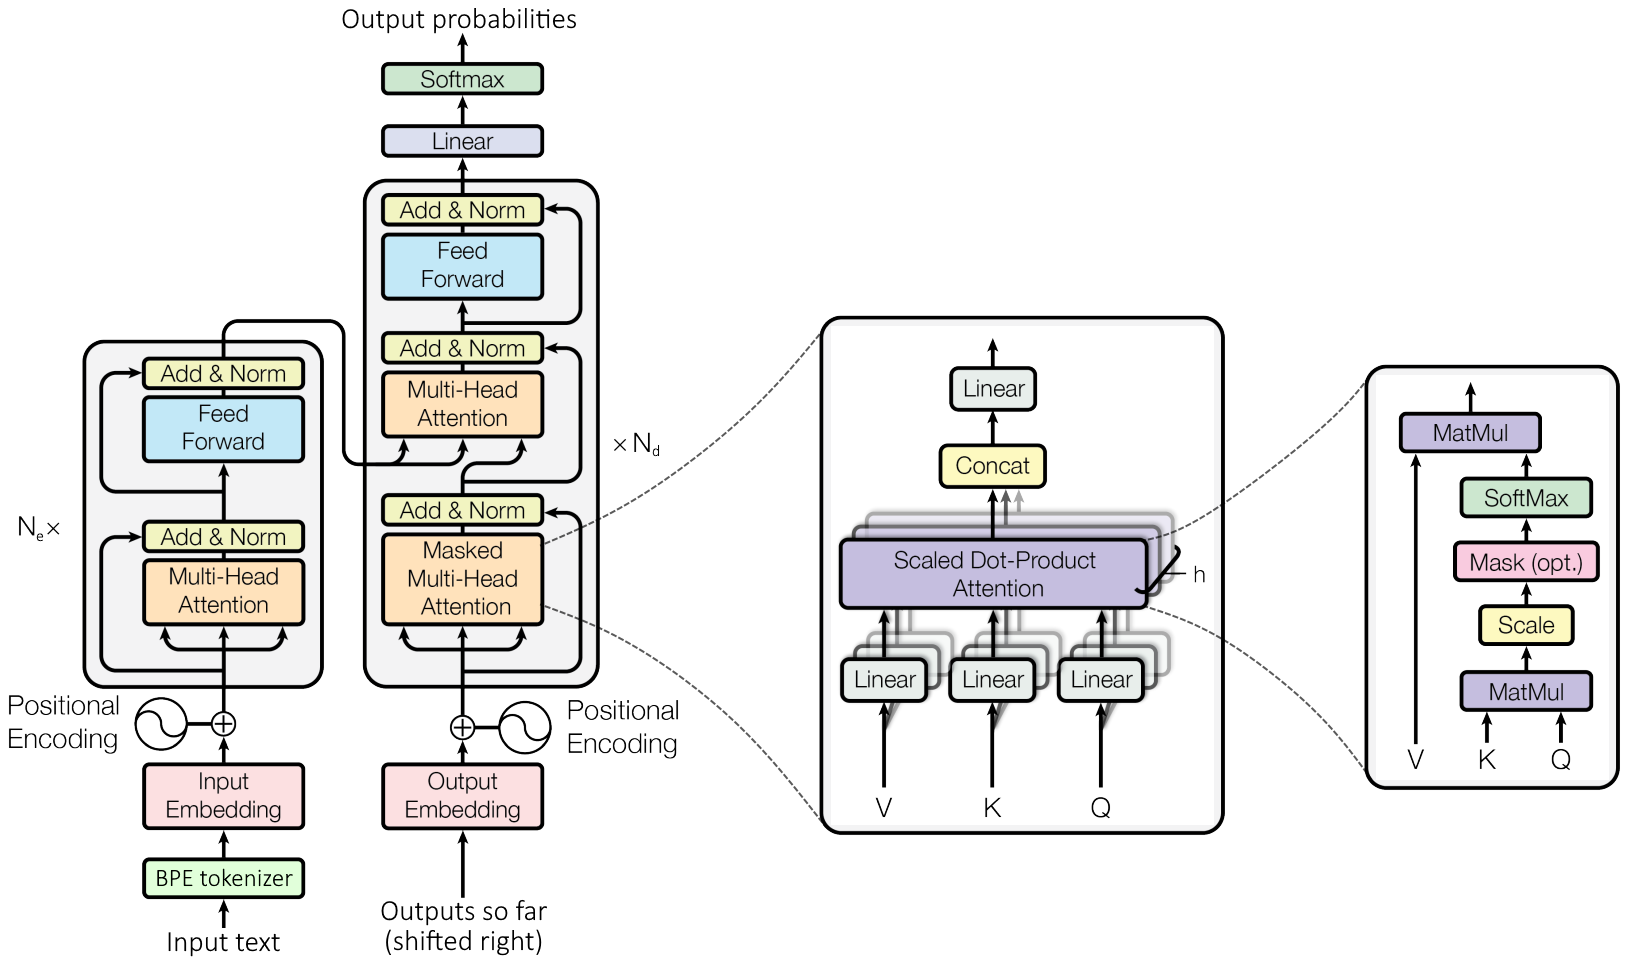
\includegraphics[width=0.75\linewidth]{res/fig/vaswani-transformer}
	\captionof{figure}{Unfloating figure}
\end{center}

\end{mdframed}

\footnotetext{This footnote text belongs to the last footnote mark that was placed.}


\begin{figure}[H]
\begin{mdframed}[backgroundcolor=black!5]
\begin{adjustwidth}{0cm}{-1cm}
\scalebox{0.8}{
\begin{tikzpicture}[
     myboxtext/.style={rectangle, draw, minimum width=1.4em, minimum height=10mm, text depth=0mm, text height=1em},  % "Text height" needed to align labels vertically https://tex.stackexchange.com/a/529480/203081
     myboxarrows/.style={rectangle, draw, minimum width=9.5mm, minimum height=10mm}
 ]
 % Inspired by https://tex.stackexchange.com/a/179753/203081
 \newcommand{\randarrow}{\tikz{
     % random direction and length
     \pgfmathsetmacro\angle{rnd*360}
     \pgfmathsetmacro\halflen{2*(rnd-0.5)*0.15 + 0.3}  % When this value is 0.5, the arrow is 10mm long.
     \draw[line width=1.25pt,-stealth,color=black] (0,0) +(\angle:-\halflen) -- +(\angle:\halflen);}
 }
 
 \def\tokens{
     \textunderscore{}Rob/3663, BER/14334, T/342, 's/167, \textunderscore{}B/138, PE/14388, -/19, to/2751, ken/859, iser/8468, \textunderscore{}split/18486, ste/369, \textunderscore{}dit/52, \textunderscore{}voorbeeld/1403, \textunderscore{}el/4241, o/169, qu/2237, ent/666, ./4
 }
 \edef\tokenAmount{0}  % No, you can't just calculate the length of the above array. I struggled for a whole hour trying to put the result of a function call that did that into a variable that would be allowed by the rectangle below.

 \def\origin{3.1em}

 \node[anchor=west] at (0,\origin) {RobBERT's BPE-tokeniser splitste dit voorbeeld eloquent.};

 \def\origin{0em}

 \node (node0) at (0,\origin) {};
 \foreach \token/\id [count=\x] in \tokens {
     \pgfmathsetmacro{\prevx}{\x-1}
     
     \node[right=-0.15mm of node\prevx, fill=white] (node\x) [myboxtext] {\token};
     \node[below=5mm of node\x.center] {\footnotesize \x};
     \xdef\tokenAmount{\x}
 }
 \draw[ultra thick] (node1.south west) rectangle (node\tokenAmount.north east);

 \def\origin{-5em}

 \node (inode0) at (0,\origin) {};
 \foreach \token/\id [count=\x] in \tokens {
     \pgfmathsetmacro{\prevx}{\x-1}
 
     \node[inner sep=0mm,right=0mm of inode\prevx, fill=white] (inode\x) [myboxarrows]  {\footnotesize\id };
     \node[below=5mm of inode\x.center]  {\footnotesize \x};
 }
 \draw[ultra thick] (inode1.south west) rectangle (inode\tokenAmount.north east);

 \def\origin{-10em}

 \pgfmathsetseed{34678901}
 \node (anode0) at (0,\origin) {};
 \foreach \token/\id [count=\x] in \tokens {
     \pgfmathsetmacro{\prevx}{\x-1}
 
     \node[right=0mm of anode\prevx, fill=white] (anode\x) [myboxarrows]  { };
     \node[below=5mm of anode\x.center]  {\footnotesize \x};
     \node at (anode\x.center) { \randarrow };
 }
 \draw[ultra thick] (anode1.south west) rectangle (anode\tokenAmount.north east);
\end{tikzpicture}
}
\end{adjustwidth}
\end{mdframed}
\caption[Data formats at the interfaces inside an NLP system]{Data formats at the interfaces inside an NLP system. Top to bottom: what the tokeniser sees (characters), what the vocabulary sees (subwords), what the embedding matrix sees (token-IDs), and what a neural model sees (embedding vectors).}
\label{fig:interfaces}
\end{figure}


\section{Code}
When you typeset code, it is a crime to use the \co{listings} package.

The \TeX{}studio settings that come with \repo allow typesetting with the \verb|minted| package out of the box. You can do this inline with the \verb|\mintinline| command, like \mintinline{python}|bytes(corpus, "utf-8")|, you can load code from a file with \verb|\inputminted| like
\inputminted[linenos]{python}{./res/code/hello.py}

and finally, if it's a very small example snippet, you can also just embed your code in the \verb|minted| environment in your \LaTeX{} document:
\begin{minted}[linenos]{python}
def example() -> int:
    return 1
\end{minted}

\section{Menus}
If, for some reason, you need to tell readers how to navigate through a digital menu, you can do so with \verb|\menu[,]{a,b,c,d,e}|. For example, my thesis contained the menu path
\menu[,]{Create Lexicon, Dutch Lemmas, StrucLab, Ok, Ok, Include Word, Ok}

\section{Controlling line breaks}
These commands are not specific to \repo, but I'll mention them anyway. \textbf{Note:} you probably shouldn't use these unless you are finished writing your thesis.
\begin{itemize}
\item If you want to force text to the next line and leave the rest of the line blank without triggering a blank line, insert \verb|\\|.
\item If you want a word to be more likely to be hyphenated at a certain point, add \verb|\-| at that point in the word. This helps in Dutch compounds, which \LaTeX{} sometimes can't hyphenate, e.g.\ \verb|rivier\-beddings\-door\-sneden|.
\item If you want to protect a word against being hyphenated at the edge of a line, surround it by \verb|\mbox{}|.
\item If you want a certain space to never be the end a line, replace it by \verb|~|.
\item If you want a certain space to be more likely to be the end of a line, replace it by \verb|\allowbreak{}|.
\item If you want a word to be able to exceed the edge of the line, use \verb|\rlap|.
\end{itemize}


\section{Todos}
Because the \co{todonotes} \LaTeX{} package is evil, \repo defines its own rudimentary \verb|\todo{...}| command that will show up as red boxes in the margin of your thesis.\todo{Like this.}
